\documentclass[12pt]{article}
\usepackage{amssymb,amsmath,latexsym,verbatim,amsthm}
\usepackage{tikz,listings,url}
\usepackage{mathtools}
\usepackage{float}
\usepackage[margin=0.5in]{geometry}
\usepackage{float}
%\usepackage{hyperref}
\usetikzlibrary{matrix,shapes,arrows,positioning,chains, calc}

\lstset{basicstyle=\bfseries\small}

\newcommand{\nbar}{\overline{n}}
\newcommand{\mbar}{\overline{m}}
\newcommand{\Z}{\mathbb{Z}}
\newtheorem{claim}{Claim}
\usepackage{array}
\newcolumntype{R}[1]{>{\raggedleft\let\newline\\\arraybackslash\hspace{0pt}}m{#1}}

\begin{document}
\title{A generalization of a reconciliation mechanism}
\maketitle

Here we focus on the even modulus, for simplicity we will assume that the modulus is a power of two (in our instantiation/implementation $q = 2^{32}$).

In the Section~\ref{sec:2bits} we describe the mechanism for extracting 2 bits (\cite{P14} describes the mechamism for extracting 1 bit) from a single ring element. In Section~\ref{sec:Bbits} we generalize the mechanism to extracting an arbitrary number of bits (as long as the noise is not too big). In Section~\ref{sec:correctness} we show how these changes affect the correctness of key exchange by upper bounding the probability for two parties to get different keys.

\section{Extracting 2 bits from a single element}
\label{sec:2bits}
Following the original idea of Peikert~\cite{P14} for element $v \in \Z_q$ we define functions
\begin{align*}
\lfloor \cdot \rceil_4: \Z_q \rightarrow \{0, 1, 2, 3\}\;\;\text{s.t.}\;\; \lfloor v \rceil_4 = \left\lfloor \frac{4}{q} x\right\rceil\\
\langle \cdot \rangle_4: \Z_q \rightarrow \{0, 1\}\;\;\text{s.t.}\;\; \langle v \rangle_4 = \left\lfloor \frac{8}{q} \right\rfloor \mod 2
\end{align*}

We define disjoint intervals $I_0 := \{0, 1, \ldots, \frac{q}{4} - 1\}; I_k := I_0 + k \cdot \frac{q}{4}$, where $k \in \{1, 2, 3\}$.
% each consisting of $\frac{q}{4}$ elements in $\Z_q$. These elements form a partition of $\Z_q$. The index of the interval $I_k$ indicates the value of $\lfloor \cdot \rceil_4$ function on that interval:
\begin{align*}
\lfloor v \rceil_4 = k\text{ iff }v \in I_k.
\end{align*}

We define disjoint intervals which are twice smaller: $J_0 := \{0, 1, \ldots, \frac{q}{8} - 1\}; J_k := J_0 + k \cdot \frac{q}{8}$, where $k \in \{1, \ldots, 7\}$.

Lets define $S_0 = J_0 \cup J_2 \cup J_4 \cup J_6$, and $S_1 = J_1 \cup J_3 \cup J_5 \cup J_7 = \Z_q \backslash S_0$.

\begin{align*}
\langle v \rangle_4 = b\text{ iff } v \in S_b,\\
%\langle v \rangle_4 = b&\text{ iff }v \in J_{b + 2k}\;\text{for some }k,\\
%I_k = J_{0 + 2k} \cup J_{1 + 2k}\;\;\text{for}\;\;k\in\{0,\ldots,3\}.
\end{align*}

The partition is shown on the picture below:
\begin{figure}[H]
    \centering
    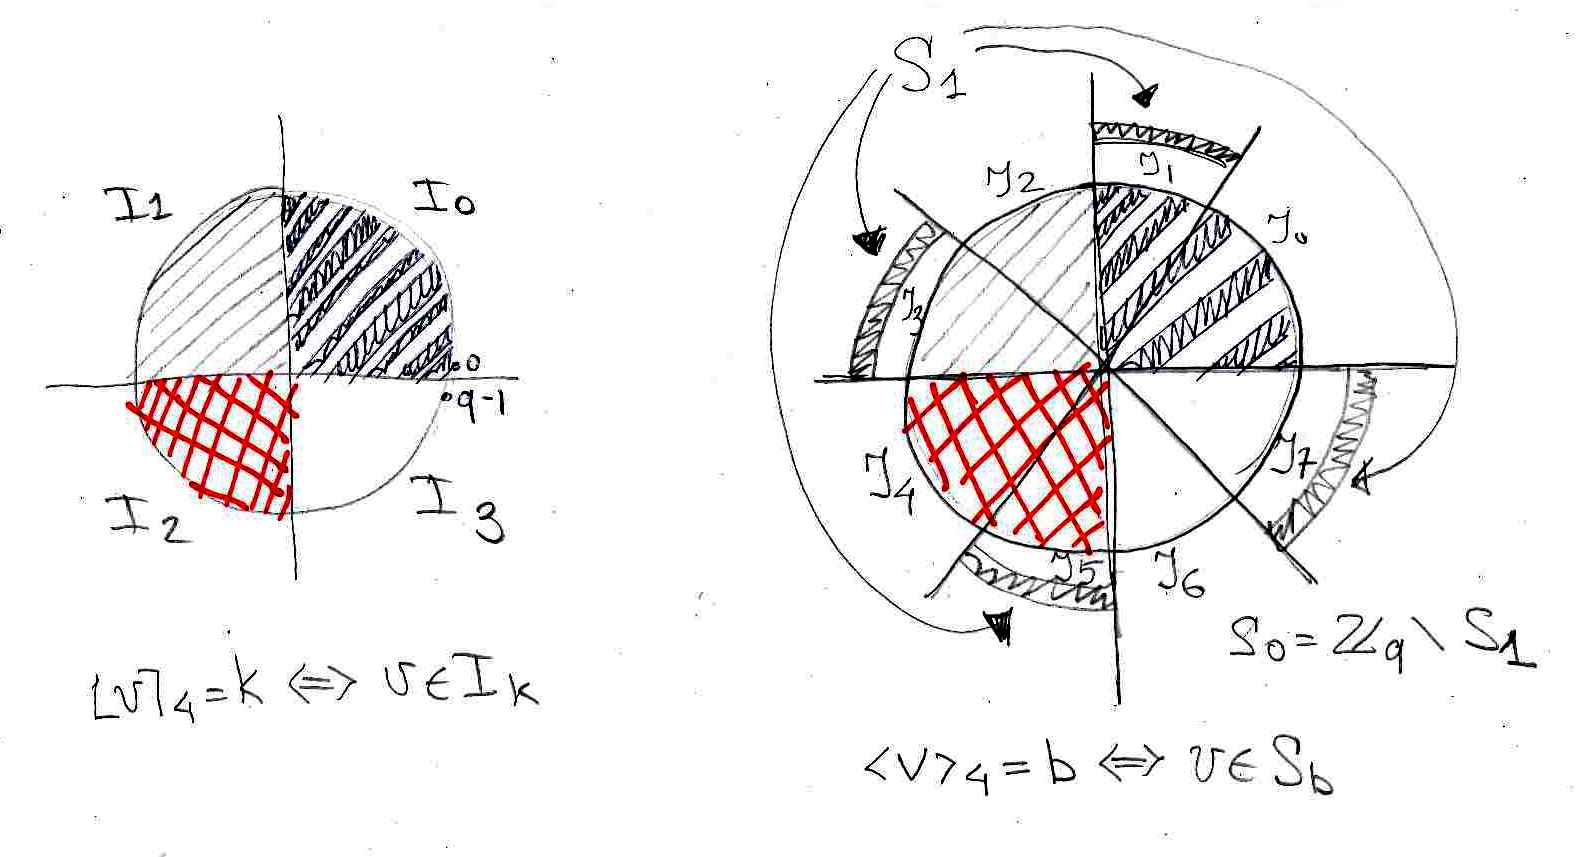
\includegraphics[width=0.8\textwidth]{2bits_pic.jpg}
\end{figure}

\begin{claim}
If $v \in \Z_q$ is uniformly random, then $\lfloor v \rceil_4$ is uniformly ramdom given $\langle v \rangle_4$.
\end{claim}
\begin{proof}
For any $b \in \{0, 1\}$, if we condition on $\langle v \rangle_4 = b$, then $v$ is uniform over $J_b \cup J_{2+b} \cup J_{4+b} \cup J_{6+b}$. If $v \in J_{b + 2k}$, then $\lfloor v \rceil_4 = k$, so $\lfloor v \rceil_4$ is uniformly random given $\langle v \rangle_4$.
\end{proof}

Define the reconciliation function $rec: \Z_q \times \{0, 1\} \rightarrow \Z_4$ as
\begin{align*}
rec(w, b):= k\text{ if } w \in J_{2k + b} + E
\end{align*}

\begin{claim}
If $w = v + e \mod q$ for $v \in \Z_q$ and $e \in E$, where $E = \left[-\frac{q}{16}, \frac{q}{16}\right) \cap \Z$, then $rec(w, \langle v \rangle_4) = \lfloor v \rceil_4$
\end{claim}
\begin{proof}
Let $b = \langle v \rangle_4 \in \{0, 1\}$, so $v \in J_b \cup J_{2+b} \cup J_{4+b} \cup J_{6+b}$. Then $\lfloor v \rceil_4 = k$ if and only if $v \in I_k$. This holds if and only if $w \in J_{2k + b} + E$, because $J_{2k + b} + E$ are disjoint for different $k$'s.
\end{proof}

\section{Extracting $B$ bits from a single element}
\label{sec:Bbits}
The approach described above can be generalized to extracting $B$ bits.
We again define functions
\begin{align*}
\lfloor \cdot \rceil_{2^B}: \Z_q \rightarrow \{0, \ldots, 2^B - 1\}\;\;\text{s.t.}\;\; \lfloor v \rceil_{2^B} = \left\lfloor \frac{2^B}{q} x\right\rceil\\
\langle \cdot \rangle_{2^B}: \Z_q \rightarrow \{0, 1\}\;\;\text{s.t.}\;\; \langle v \rangle_{2^B} = \left\lfloor \frac{2^{B+1}}{q} \right\rfloor \mod 2
\end{align*}

We again define $2^B$ intervals $\{I_k\}$ and $2^{B + 1}$ intervals $\{J_{2k + b}\}$ such that
\begin{align*}
\lfloor v \rceil_4 = k&\text{ iff }v \in I_k,\\
\langle v \rangle_4 = b&\text{ iff }v \in J_{b + 2k}\;\text{for some }k.
\end{align*}
The case of $B = 3$ is shown on the picture below:
\begin{figure}[H]
    \centering
    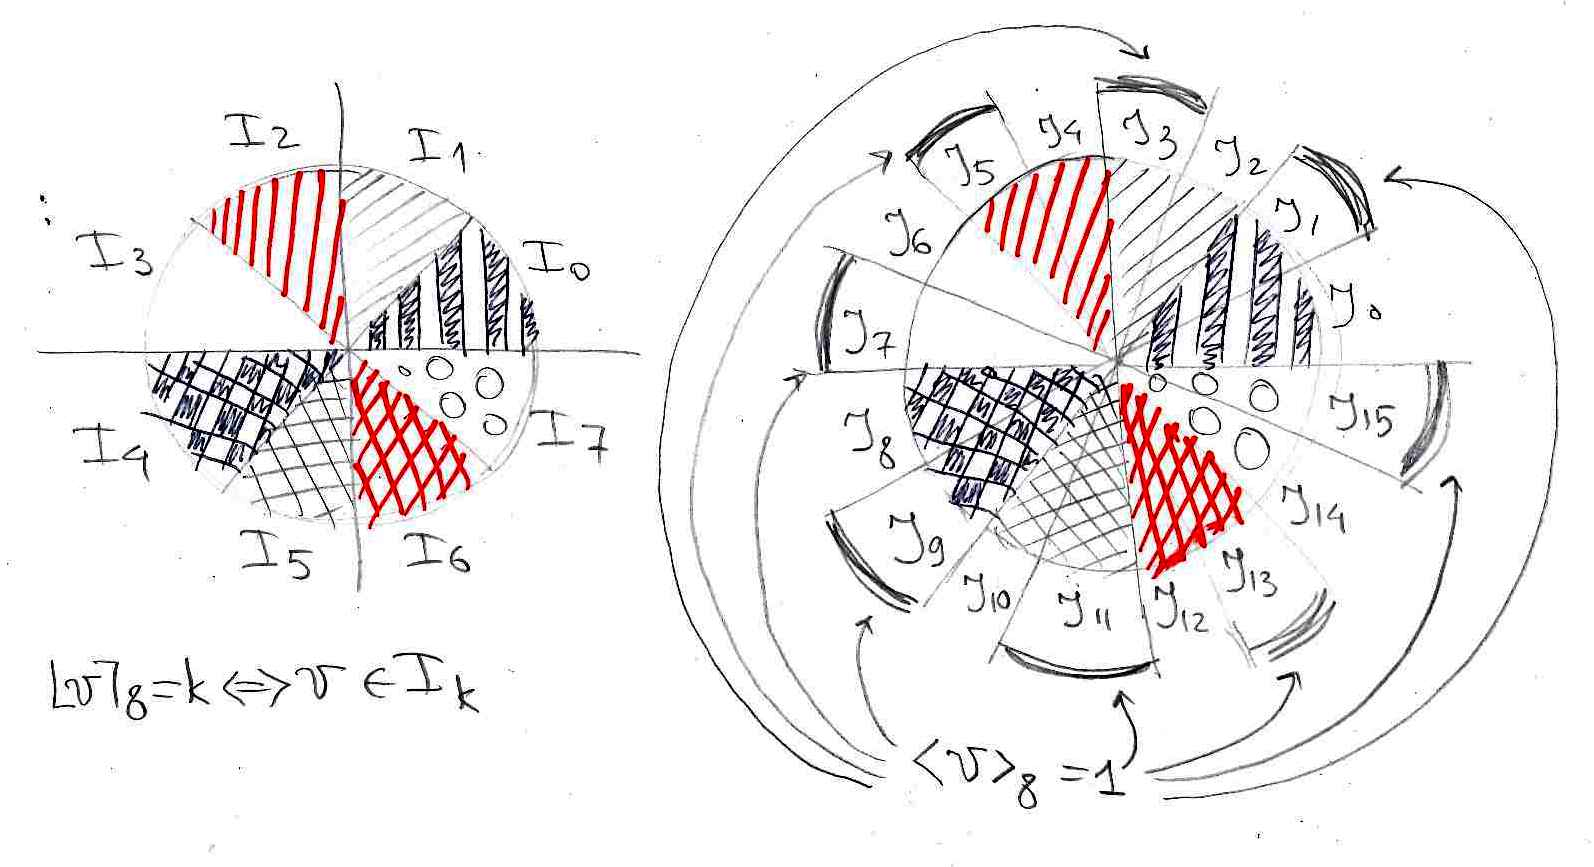
\includegraphics[width=0.8\textwidth]{3bits_pic.jpg}
\end{figure}

Similar claims can be proven for $E = \left[-\frac{q}{2^{B+2}}, \frac{q}{2^{B+2}}\right) \cap \Z$.

\section{Correctness for key exchange mechanism}
\label{sec:correctness}
For correctness we require that for all pairs of indices $(i, j)$, $|(E'S + S'E + E'')_{ij}| < \frac{q}{2^{2 + B}} - \frac{1}{2}$. Here $S,E \in \Z_q^{n \times \nbar}$, $S', E' \in \Z_q^{\mbar \times n}$, $E'' \in \Z_q^{\mbar \times \nbar}$ and they all are draw from a Gaussian distribution with standard deviation $\sigma$.
For a fixed pair $(i, j)$, we bound the probability of $|(E'S + S'E + E'')_{ij}| > \frac{q}{2^{2 + B}} - \frac{1}{2}$ as follows. There are $2n + 1$ terms in the sum, if the $(ij)$ element is greater than $\frac{q}{2^{2 + B}} - \frac{1}{2}$, then at least one of the elements of the gaussian matrix must exceed $z = \sqrt{\frac{q}{2^{2 + B} (2n + 1)}}$ in absolute value. The probability of individual gaussian coefficient exceeding $z$ in absolute value can be bounded by $e^{-(z / (\sqrt{2}\sigma))^2}$. The probability that one out of (4n + 1) exceeds $z$ is bounded above by the sum $(4n + 1)e^{-(z / (\sqrt{2}\sigma))^2}$. Similarly, the probability that at least one coefficient of $k_A$ and $k_B$ disagree is clearly bounded above by the sum of all the $p_{ij}$, so we get
\begin{equation}
\Pr(k_A \neq k_B) \leq \sum_{i = 0}^{\nbar} \sum_{j = 0}^{\nbar} p_{ij} \leq \nbar \cdot \mbar (4n + 1)e^{-q/ (2 \cdot 2^{2 + B} (2n + 1)\sigma^2)}
\label{eq:correctness_2_alternative}
\end{equation}

For our choice of parameters: $q = 2^{32}$, $n = 1024$, $\nbar \cdot \mbar = 128$, $\sigma = 3.2$, for different numbers of extracted bits the decay in this probability is shown in the table below:
\begin{align*}
(\nbar \cdot \mbar) (4n + 1)e^{-q/ (2 \cdot 2^{2 + B} (2n + 1)\sigma^2)} =\\
2^7 \cdot 2^{12} \exp\left(-\frac{2^{32}}{2^{3 + B} \cdot 2^{11} \cdot \sigma^2}\right) =\\
2^{19} \exp(-2^{18 - B} / \sigma^2) =\\
10^{\log_{10}2 \cdot 19 - \log_{10} e \cdot 2^{18 - B} / \sigma^2}
\end{align*}
\begin{center}
    \begin{tabular}{|R{3cm}|r|}
    \hline
    Bits extracted from one ring element ($i$) & Probability of failure\\ \hline
    1 & 1e-5553\\ \hline
    2 & 1e-2773\\ \hline
    3 & 1e-1384\\ \hline
    4 & 1e-689\\ \hline
    5 & 1e-341\\ \hline
    6 & 1e-167\\ \hline
    7 & 1e-81\\ \hline
    8 & 1e-37\\ \hline
    9 & 1e-15\\ \hline
    10 & 1e-5\\ \hline
    11 & 1e1\\ \hline
    \end{tabular}
\end{center}

Note: 1e-x stands for $10^{-x}$.

The parameters of the scheme scale as $\frac{1}{\sqrt{B}}$.


\bibliographystyle{alpha}
\bibliography{WriteUp}

\end{document}
